\chapter{Introduction}
\label{sec:intro}

- mention phototoxicity early on

Fluorescence microscopy is an old technique that has been established    \cm{why fluorescence microscopes}
in live sciences for a long time. Being able to see things happening
at the micrometre scale is the fundamental path to understand life and
disease.

Innovation continuously improves microscopy and occasionally new        \cm{it continues to improve}
fields of research are opened up: The discovery and development of
fluorescent proteins initiated a revolution in how microscopy can be
applied in living specimen. 

Optical high resolution techniques allow to observe biological          \cm{recently high res}
processes at the scale of individual molecules (tens of nm).

Labels that report membrane potentials or viscosity within cells,       \cm{labelling, switching}
compounds that locally release chemicals when illuminated by light or
even ion pumps that can be switched by light promise novel interesting
research.

All these techniques have in common, that excitation light has to       \cm{phototoxicity}
reach a focal point, line or plane within the sample. For this the
light has to traverse a more or less dense distribution of
fluorophores.  With few exceptions (2-photon, SPIM) microscopes are
generally not optimized for exciting only the in focus fluorophores.

- insert biological problems

- screening for medication against pathogens

- embryological development

\figref{fig:celegans-devel} compares time lapse experiments on three    \cm{embryo example}
different \emph{Caenorhabditis elegans} embryos with varying
illumination intensities. These are small invertebrates. The adult
form is approximately \unit[1]{mm} long . Their anatomy and normal
development are comparatively simple and have been well characterized
\citep{Durbin1987}.

- move the details into extra chapter

The lineage tree of two developing \emph{C. elegans} embryos is the     \cm{reproducible development}
same.  Even the number of somatic cells is constant in the organism
(959). With all other factors being equal, particularly the
temperature constant at room temperature (21\pm1 FIXME), two different
embryos will develop at the same speed from egg to fertile adult in
three and a half days. This makes the following experiment possible,
which has been conducted by Jean-Yves Tinevez at Institut Pasteur.

Embryos are removed from their mothers at an identical stage, before    \cm{description of experiment}
any cellular divisions have occured. A $z-$stack of the egg with 41
slices and $\unit[1]{\mu m}$ $z-$sampling is obtained every 2 minutes
of the egg.

Each column in \figref{fig:celegans-devel} shows an embryo at the     \cm{effect of different intensitites}
beginning, after one hour and after two hours and 38 minutes of
development. The left embryo was illuminated with only 0.5\% of the
maximum illumination intensity possible (controlled by AOTF). The
middle embryo was illuminated with 5\% and for the right embryo an
excitation power of 20\% was used.

The images show maximum intensity projections of the $z-$stacks and     \cm{description of images}
each image was normalized so that its darkest pixel is black and its
brightest pixel is white. Comparing the images in the top row from the
start of the development the left image\footnote{Note, that the left
  image in \figref{fig:celegans-devel} is the noisiest in the top
  row. This is due to the photon shot noise, which is Poisson
  distributed.} contains the least amount of fluorescence photons and
the right image the most.

One hour into the experiment, we observe that the right embryo with
the highest excitation dosage died and its fluorophores were bleached.
Some cells even turned apoptotic and went into programmed cell death.

After two hours and 38 minutes the left embryo, that received the
lowest dosage, has developed the most cells. The middle embryo ceased
developing. Reactive oxygen species created by Cells in presence of
reactive oxygen species under oxidative stress activate a DNA damage
checkpoint and arrest their cell cycle progression so as to allow for
repair and prevention of the transmission of damaged or incompletely
replicated chromosomes. The right embryo died much earlier and nearly
all its fluorophores are bleached at the end of the experiment.

% Molecular mechanisms of mammalian DNA repair and the DNA damage
% checkpoints. Aziz Sancar Stuart Linn


It should be noted, that the embryos themselves do not produce the    \cm{constant reservoir of GFP}
fluorescent proteins themselves. Already in the parent the egg
contains a certain amount of histone-2B proteins, some of which is
tagged with the green fluorescent eGFP protein. The histones are
components of the chromatin. Therefore the images in
\figref{fig:celegans-devel} label the cell nuclei.

It is useful that the egg stays at constant size within a diameter   \cm{size constant}
of approximately $\unit[60]{\mu m}$.

\begin{figure}[!htb]
  \centering
  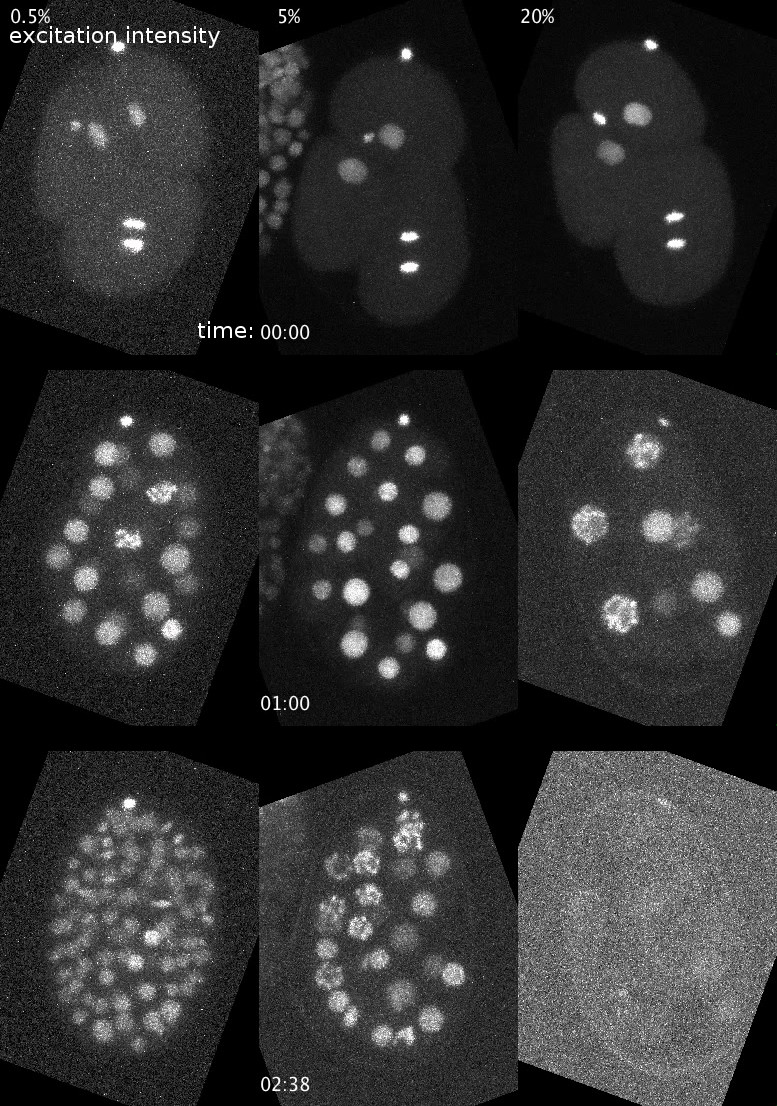
\includegraphics[width=12cm]{celegans-devel}
  \caption{Phototoxic effects while imaging the embryonal development
    of three \emph{C.~elegans} embryos (strain AZ212, histone-2B
    tagged with eGFP) with different excitation intensities. The
    embryo with lowest excitation dosage (left) develops fastest. The
    embryo with the highest dosage (right) ceases development and
    nearly all fluorophores are bleached after the experiment. Images by
    J.-Y. Tinevez (Institut Pasteur, Paris).}
  \label{fig:celegans-devel}
\end{figure}


In the rest of this chapter we give an overview of the photophysics of
fluorophores. We inicate why oxygen is such an important component in
the process of photobleaching and phototoxicity.  Then we give an
introduce conventional microscopes and finally we describe the noise
sources of CCD cameras.

\begin{figure}[!htb]
  \centering
  \pdfinput{3.5in}{worm-survival}
  \caption{dfakj}
  \label{fig:worm-survival}
\end{figure}

\section{Fundamentals of fluorescence}
\begin{summary}
  Here we give a short overview of the field of fluorescence of
  molecules in order to introduce the terms Stokes' shift, triplet
  state and photobleaching.
\end{summary}
\subsection{Construction of molecular orbitals}
First we consider a very simple molecule: We move the nuclei of two
hydrogen atoms and move them slowly together. When the nuclei have a
big distance, the atoms exist as two separate entities without
influence on each other.
\begin{figure}[!hbt]
  \centering
  \input{flu-potential_my.eps_tex}
  \caption{Schematic electron density maps and potential curves for
    ground state $\H_2$ and excited state $\H_2^*$ of molecular
    hydrogen and the cation $\H_2^+$ of molecular hydrogen
    \citep[inspired from][p.~258]{Haken2006}.}
  \label{fig:flu-potential_my}
\end{figure}

For internuclear distances in between these two extremes, we express
molecular orbitals as a linear combination of atomic orbitals and
calculate their potential energy in dependence of the distance between
the nuclei (see \figref{fig:flu-potential_my}). The curve for
$\sigma_g\sigma_g^1\Sigma_g^+$ is minimal at a internuclear distance
$R$ of approximately 1.3 Bohr radii
($a_H=\unit[0.529\cdot10^{-8}]{cm}$). The compound of two protons and
two electrons is particularly stable for this distance. We call it the
hydrogen molecule $\H_2$.

Likewise a linear combination of the atomic orbitals of a ground state
hydrogen atom $\H$ with an excited hydrogen atom $\H^*$ lead to the
molecular orbital $\sigma_g\pi_u^1\Pi_u$. There, a minimum in the
potential occurs at an increased internuclear distance (bond
length). The excited atomic orbital has a reduced probability density
close to the nucleus but similar electron--electron
repulsion. Therefore the strength of the molecular bond (order of the
bond) is reduced.
\newcommand{\vmu}{\mbox{\boldmath{$\mu$}}}
\subsection{Absorption and emission of light}
A transition between a ground state $S_0$ to an excited state $S_1$
occurs, when a radiation field connects the two states. The connection
is described by the transition dipole moment
$\vmu_{0\rightarrow 1}$.
\begin{align}
  \vmu_{0\rightarrow 1} &= \int \psi^*_0 \vmu \psi_1 \textrm{d}^3\r
\end{align}
where $\psi_0$ and $\psi_1$ are wavefunctions for the ground and
excited state, respectively \citep{Klessinger1989}.

An incident photon can electronically excite a molecule from the
highest occupied molecular orbital (HOMO), usually the singlet ground
state $S_0$, into the lowest unoccupied molecular orbital (LUMO), the
singlet excited state $S_1$.\nomenclature{HOMO}{highest occupied
  molecular orbital}\nomenclature{LUMO}{lowest unoccupied molecular
  orbital} For this, the energy $E_\textrm{ph}=hc/\lambda$ of the
photon has to match the energy gap $\Delta E=E_{S_1}-E_{S_0}$ of a
possible electronic transition within the molecule (Bohr's frequency
condition).

Photons with wavelengths below \unit[200]{nm} have sufficient energy
to ionize molecules. On the other side of the spectrum, a dye that
absorbs in the near-infrared ($\unit[>700]{nm}$) has a low-lying
excited singlet state $S_1$ and potentially increased reactivity
\citep{Sauer2011}. Hence, most known stable and bright fluorophores
absorb and emit in the wavelength range between \unit[300]{nm} and
\unit[700]{nm}.

As opposed to atomic spectra the absorption bands of organic dyes
usually span several tens of nanometers\footnote{Note that wavelength
  isn't a convenient unit to characterize absorption bands. Rather one
  should use energy or wavenumbers.}. This is because dye molecules
are composed of many atoms and this structure can vibrate, rotate and
interact with the solvent.
\subsection{Vibration of molecules}
The distance between the two nuclei of the hydrogen molecule is not
rigid. The nuclei can oscillate around their position of equilibrium
at quantized frequencies. The vibration frequencies depend on the
order of the bond and the mass of the two nuclei. When a molecule is
electronically excited, its vibration frequencies decrease.
\begin{figure}[!hbt]
  \centering
  % (423-120)/423*7 = 4.77 ,trim=0 0 135 0,clip
  \input{flu-condon_my.eps_tex}
  \caption{Illustration of the Franck-Condon principle. Potential
    curves for either the same bond length in the
    excited state ({\bf left}) or a larger bond length in the
    excited state ({\bf right}). Electronic transition occurs
    instantaneously and excites higher vibro-rotational states in the
    right diagram. \citep[inspired from][p.~276]{Haken2006}.}
  \label{fig:flu-condon}
\end{figure}

\figref{fig:flu-condon} schematically shows potential curves for the
ground state $S_0$ and the first excited state $S_1$ of two different
molecules. The left graph depicts a molecule where the internuclear
distance is the same in the ground $S_0$ and excited $S_1$ stage. When
such a molecule absorbs a photon, its electron is excited but its
vibrational mode does not change. The anthracene molecule shows such
behaviour.

The right graph depicts a molecule that has a larger internuclear
distance in its excited state. When a photon is absorbed, the
electronic state of the molecule transitions into the higher state
$S_1$. The mass of the electron is much smaller than the
nucleus. Therefore the electronic transition takes place in a
timescale of $\unit[\sim10^{-15}]{s}$. In this duration the nuclei do
not move (\emph{Born-Oppenheimer approximation}: electronic
transitions occur as if the nuclei were fixed in place). The changed
bond length with the new orbital of the excited state $S_1$ drives the
nuclei into movement (excitation of vibro-rotational modes,
\emph{Franck-Condon principle}: electronic transition most likely
occurs without changes to the position of the nuclei and the intensity
of a vibrational transition depends on the overlap between the
vibrational wavefunctions).

\subsection{Depopulation pathways of excited states}
\begin{figure}[!hbt]
  \centering
  \def\svgscale{.8}
  {\small
  \input{flu-level_my.eps_tex}}
  \caption{A typical energy level diagram. The boxes depict orbitals,
    up and down arrows symbolize the spin of the outer electrons. Fat
    lines represent electronic states. Thinner lines indicate
    vibro-rotational states. Various processes are shown with their
    typical time scales. VR = vibro-rotational relaxation, ISC =
    intersystem crossing, IC = internal conversion \cite[inspired
    from][]{Haken2006}.}
  \label{fig:flu-level}
\end{figure}
The Jablonski diagram in \figref{fig:flu-level} summarizes information
about the energy levels of a molecule and possible transition
processes. If a molecule is in the ground state $S_0$ one of its outer
electrons can be excited by absorbing a photon to the first excited
singlet state $S_1$.  If the photon has an even higher energy, the
electron will go into the second excited singlet state $S_2$.

Transition from the ground state into higher electronic states than
$S_2$ is not usual in commonly used fluorophores and wavelength range.
Absorption of one photon doesn't change the spin of an electron and
therefore the transition $S_0\rightarrow T_1$ into the triplet state
$T_1$ only occurs with very low probability.

\subsubsection{Kasha's rule}
As described above, electronic excitation in general also leads to the
excitation of a vibro-rotational nonequilibrium state (Franck-Condon
state). In microscopy, fluorophores are often in solution, where they
experience at least $10^{12}$ collisions per second. Inter- and
intramolecular interactions bring the vibrations of the fluorophore
molecule back to thermal equilibrium\footnote{Rotation states have
  energies corresponding up to \unit[100]{$cm^{-1}$} (microwave),
  vibration states have energies corresponding to wavenumbers from 300
  to \unit[3000]{$cm^{-1}$} (infrared). Electronic states have
  energies in the visible. The number of excited molecules in thermal
  equilibrium is governed by the Boltzmann law and proportional to
  $\exp(-\Delta E/(k_BT))$. Therefore, at room temperature ($k_B
  T\sim\unit[200]{cm^{-1}}$), only rotation states are excited. } in a
very short timescale ($\unit[10^{-12}]{s}$). This is considerably less
then the lifetime of the electronic excitation (few
nanoseconds). Therefore spontaneous emission of a photon will occur
from the vibrational ground state $S_{1,v_1=0}$ (\emph{Kasha's rule}).

\subsubsection{Stokes' shift}
During emission of a fluorescence photon a Franck-Condon state of the
singlet ground state $S_0$ is excited and returns into thermal
equilibrium by vibro-rotational relaxation. Thus, some of the energy
of the original excitation photon is lost as heat. The emitted
fluorescence photon is red shifted compared to the excitation
photon. Technically the \emph{Stokes' shift} is defined as the
difference of the wavenumbers of the fluorescence maximum and
absorption maximum\footnote{Sometimes the Stokes' shift is also defined
  as the distance of the absorption maximum to the point where the
  normalized absorption and corrected fluorescence emission curves intersect.}.

In terms of wavelength the Stokes' shift usually corresponds a change
of 15 to \unit[30]{nm}. The Stokes' shift is bigger, when the shape and
position of the potential of the excited state $S_1$ differs from the
ground state $S1$ (see \figref{fig:flu-condon}, right). There are
fluorophores with more than \unit[100]{nm} Stokes shift.

\subsubsection{Internal conversion}
Often the transition $S_2\rightarrow S_1$ occurs by \emph{internal
  conversion} (IC) followed by vibro-rotational relaxation. During IC,
the electronic state transitions into a high vibro-rotational
excitation of a lower electronic state. The probability for IC is high
for a high density of vibrational target states.
% FIXME translate Zustandsdichte

For floppy, non-rigid molecules, IC is a competing process to
fluorescence $S_1\rightarrow S_0$. In dyes that absorb in the near
infrared, the energy gap between $S_0$ and $S_1$ is so small and the
vibrational states of highest energy of the singlet ground state $S_0$
(vibration of hydrogen bonds directly attached to the chromophore) are
close to $S_1$. This seriously reduces the efficiency of infrared dyes
\citep[p.~43]{Sauer2011}.


\subsubsection{Fluorescence quantum yield}
The \emph{fluorescence quantum yield} $\eta$ of a fluorophore is
defined as the quotient of the number of emitted (fluorescence)
photons and the number of absorbed photons. In dyes like rhodamine~6G
(in ethanol $\eta=0.94$ \cite{Fischer1996}) or anthracene
(9,10-diphenyl anthracene in cyclohexane $\eta=0.90$ \cite{Hamai1983})
its value can be nearly 1 in an appropriate solvent.


\subsubsection{Intersystem crossing}
There is a small probability that the HOMO electron doesn't relax by
internal conversion or emission of a fluorescence photon. Instead it
flips its spin (due to spin-orbit coupling\footnote{The probability of
  a spin flip is increased if heavier atoms are part of the
  molecule. E.g.\ while fluorescein has a triplet yield of 0.03, the
  triplet yield of eosin, a fluorescein derivative with four bromine
  substituents is 0.76 \citep[p.~37]{Sauer2011}.}). This process is
called \emph{intersystem crossing} and populates the first triplet
state $T_1$. A transition into the ground state $S_0$ would need
another spin-flip of the electron and is quite improbable. Therefore
the triplet state has a long lifetime (up to several seconds). The
radiative decay is called phosphorescence.
  

\subsection{Photobleaching and phototoxicity}
The prolonged lifetime of the triplet state $T_1$ increases the
probability for the excited molecule to collide with a partner and
react.

\begin{figure}[!hbt]
  \centering
  \input{oxygen.eps_tex}
  \caption{{\bf left:} Molecular orbitals of the oxygen molecule. {\bf
      right:} Molecular oxygen has the lowest energy in its triplet
    state ${}^3\Sigma$. Then the spins of the two $\pi^*-$electrons
    are parallel. Inspired from \citet{Linde2011a}.}
  \label{fig:oxygen}
\end{figure}


The ground state of the oxygen molecule is a triplet state ${}^3\O_2$,
with two unpaired electrons of parallel spin in its
$\pi^*-$orbitals\footnote{The antibonding molecular orbital $\pi^*$ of
  molecular oxygen is constructed by linear combination of two atomic
  orbitals of oxygen.}  (see \figref{fig:oxygen}). The triplet ground
state and its abundance in typical microscope samples are the reasons
why oxygen is so important when it comes to phototoxicity. If an
oxygen molecule comes into physical contact with a $T_1$ fluorophore,
e.g.\ ${}^3\textsf{Chlorophyll}^*$, the energy of the dye can be
transferred to the oxygen by an electron exchange energy transfer
mechanism in which the orbitals directly interact with each other
\citetext{\citealp[p.~438]{Haken2006} and \citealp{Linde2011a}}:
\begin{align}
  {}^3\O_2 + {}^3\textsf{Chlorophyll}^* \rightarrow
  {}^1\O^*_2+{}^1\textsf{Chlorophyll}
\end{align}
This reaction is also known as triplet--triplet annihilation.  There
are two forms of singlet oxygen, that form in competition: The lower
energy ${}^1\Delta$ and the short-lived, higher energy ${}^1\Sigma$
form ($T_{1/2}\sim\unit[10^{-9}]{s}$), with spin orientations as
depicted on the right of \figref{fig:oxygen}. During the transition
${}^1\Sigma\rightarrow{}^1\Delta$ an infra-red photon with
\unit[1268]{nm} wavelength is emitted \citep[p.~20]{Linde2011a}.

The resulting singlet oxygen ${}^1\Delta$ is very reactive. In a
typical specimen it diffuses only a few tens of nanometre until it
reacts with another molecule \citep{Sauer2011}. When it reacts with
the fluorophore, it can destroy it (photobleaching) also the singlet
oxygen can damage the DNA of living creatures. Plants have developed
several protection mechanisms against being exposed to too much
light. Within the cells they reorient and shift their chloroplasts in
order to expose them to less light \citep{Reshak2009}.  However, they
even have a molecular protection mechanism: They transfer the energy
of the chlorophyll onto carotenoid molecules and can prevent the
hazardous \emph{phototoxicity} effects of singlet oxygen
\citep{Krieger-Liszkay2005}.

Nowadays many methods are known to reduce photobleaching. Substitute
oxygen with noble gases or remove it enzymatically
\citep[p.~89]{Sauer2011}. Depopulate the triplet state by adding
reducing as well as oxidizing agents to the solvent
\citep{Vogelsang2008} or couple a triplet quencher directly to the
fluorophore \citep[p.~19]{Sauer2011}. For fixed samples it helps to
change the solvent or polymer.

In living specimen these techniques may reduce photobleaching, but
they can also have an effect on the biological system itself. Removing
oxygen will quite certainly have a negative effect. In order to reduce
phototoxicity it makes sense to think about the light management in
the microscope.


\section{Conventional microscopes}
\begin{summary}
  Microscopes that are in common use today do not optimally excite
  fluorophores within the specimen. In this section we outline how
  these microscopes work. We explain how out-of-focus blur severely
  limits the performance of the wide field microscope. Then we discuss
  how confocal microscopy improves the sectioning capability at the
  cost of increasing the phototoxic load on the specimen.
\end{summary}
The basic building block of microscopes are lenses. A lens is a piece
of glass with two polished spherical surfaces. Aspherical lenses also
exist but are much harder to manufacture because of their lower
symmetry. Light is slower in glass than in air. The shape of a lens
redirects photons and the thickness of the material can delay them. A
lens ideally focuses a parallel beam of light into a spot on its focal
plane. The distance between focal plane and the region where the rays
start to converge is called focal length and denoted by $f$.
\begin{figure}[!hbt]
  \centering
  \input{widefield-microscope.eps_tex}
  \caption{{\bf a)} Schematic of a modern microscope. The sample is in
    the front focal plane of the objective. The detection tube lens
    TL1 forms a magnified image on the camera. {\bf b)} Parallel laser
    epifluorescence excitation. The excitation tube lens focuses a
    laser into the back focal plane (BFP). The beam is reflected by a
    dichromatic beam splitter (BS) towards the objective. An extended
    area in the specimen is illuminated. Fluorescence light of lower
    wavelength returns through the objective, is transmitted through
    BS and forms an image on the camera. {\bf c)} Confocal
    microscope. A pinhole PH2 is imaged as a diffraction limited spot
    into the specimen. Returning fluorescence light is only detected
    when it passes through an aligned pinhole PH1. This configuration
    rejects light that doesn't originate from the front focal plane
    (green) of the objective.}
  \label{fig:widefield-microscope}
\end{figure}

The uncoloured beam in \figref{fig:widefield-microscope}~a) represents
rays that start from the intersection $O$ of the optical axis and the
front focal plane of the objective. The objective collects the rays
and collimates them into a beam that is parallel to the optical
axis. After traversing the tube length $f+f_\textrm{TL}$, the rays are
focused by the detection tube lens TL1 on the intersection $O'$ of its
focal plane and the optical axis. 

The blue beam corresponds to rays that start from an off-axis point
$P$ in the front focal plane of the objective. Behind the objective
the blue beam is a parallel beam. However, the beam is tilted relative
to the optical axis. The tube lens TL1 focuses the blue beam into a
spot at $P'$ on its focal plane.

The objective fulfils the Abbe sine condition -- it is aplanatic. The
microscope forms stigmatic\footnote{An imaging system collects some of
  the rays, that leave an object and directs them towards the
  image. If all rays that leave an object point converge in the
  conjugate image point, then we call the image point stigmatic.}
images of points from the front focal plane in the plane perpendicular
to the optical axis, containing $O'$ and $P'$. The plane with the
images is called intermediate image plane. It is magnified by the
factor $M$:
\begin{align}
  M=\frac{\overline{O'P'}}{\overline{OP}}=\frac{f_\textrm{TL}}{f}.
\end{align}
In our microscope we use an objective with magnification $M=63$. The
focal length of the tube lens is \unit[164.5]{mm} for most Zeiss
microscopes. Therefore the focal length of our objective is
$f=\unit[2.61]{mm}$.

Let's assume we have an opaque sample with just two small
($\diameter<\unit[120]{nm}$) holes with $\unit[2]{\mu m}$ distance
between them.  We put this object into the front focal plane of the
objective and position a camera on $O'$. When illuminating the mirror
from the side opposite to the objective, the camera will show two
spots with $\unit[126]{\mu m}$ distance.

\nomenclature{NA}{numerical aperture}

Note that \figref{fig:widefield-microscope} depicts a \emph{thin-lens
  model of a high numerical aperture objective} that fulfils Abbe's
sine condition. A real objective contains in the order of ten coated
lenses of different glass and crystalline materials. Their curvatures,
positions and materials were all carefully chosen, taking into account
manufacturing tolerances and wavelengths, so that the microscope
behaves as the thin-lens model predicts. Diffraction at the periphery
of the pupil in the back focal plane dictates the resolution, one can
achieve inside of the sample.

It is quite possible that heating to \unit[37]{${}^\circ$C} will ruin
such a high-precision instrument. A related source of aberrations
(departure of design performance) is the refractive index inside of
the specimen. In Appendix~\ref{sec:ray-aberration} we describe a more
complicated model that can predict the effect of embedding the sample
in water (instead of immersion oil with the same refractive index as
the glass).

\subsection{Widefield epifluorescence microscope}
Fluorescence photons are emitted in all directions, independent of the
original illumination direction. Therefore it is possible and
convenient to use the objective for excitation as well as
detection. This mode of microscopy is called epifluorescence (Greek:
$\varepsilon\pi\iota$; on, above).  In this configuration usually only
a small percentage of the excitation light returns due to diffraction
or reflection. This simplifies the separation of fluorescence light
from excitation light.  Furthermore parts of opaque specimen can be
imaged and it is beneficial that the illumination needs to be aligned
only once.

\nomenclature{BFP}{Back focal plane}

The red beam in \figref{fig:widefield-microscope}~b) is a parallel
laser. The excitation tube lens TL2 focuses the beam into the back
focal plane (BFP) of the objective. The beam is reflected at a
dichromatic beam splitter (BS). This is a glass plate that has been
coated with dielectric layers. The refractive index, thickness and
sequence of the layers are designed so that the excitation light is
reflected towards the objective. Excitation light, that is scattered
or reflected in the sample and returns through the objective is
reflected towards the light source. However, lower energy fluorescence
light returning from the objective is transmitted towards the
camera. Behind the objective the beam is parallel and illuminates the
specimen. The field of view is the demagnified diameter of the laser
beam before TL2.
\subsubsection*{Non-uniformity due to coherent interference}
Note that tiny dirt particles and coherent interference in laser beams
can produce unwanted non-uniformities in the illumination. As a remedy
the spatial coherence of the laser is sometimes reduced.  Incoherent
light emitting diodes, mercury or xenon arc lamps are often used
instead of lasers. In the latter case a band pass filter selects the
useful part of the spectrum of the excitation lamp upstream of the
dichromatic beam splitter.

\subsubsection{Out-of-focus blur}
However, independent of the choice of the light source, the wide field
microscope in epifluorescence configuration exposes many layers of the
sample. This leads to fluorescence of out-of-focus fluorophores.

There are two reasons, why out-of-focus fluorophores give blurred
images. Not even an ideal imaging system -- a device that forms
%% FIXME refer to maxwell or born/wolf
stigmatic images of all the points in one volume in another volume --
would form sharp images on the camera plane. After all, the camera is
just a plane and the object under observation is three dimensional.

Furthermore a microscope is far from being an ideal imaging system. In
a microscope it is not possible to obtain a sharp image of a different
slice of the object by changing the axial position of the camera
behind the tube lens TL1 \citep{Botcherby2007,Botcherby2008a}.
\subsubsection*{Deconvolution}
When a stack of several slices of an object is obtained, it is
possible to suppress the blurred part of each image in all the
others. These algorithms (deconvolution) can improve the perceived
quality of images in some stacks. However, there are two fundamental
problems:

First the \emph{missing cone problem} prevents focusing on a
homogeneous fluorescent plane. Physics dictates that there is always a
gap in the transfer function of the objective when the fluorescence
process is linear and the objective collects only photons from one
half space (see \figref{fig:missing-cone}). Not all spatial
frequencies within the transfer function attenuate with defocus
\citep{Neil1997}.

\begin{figure}[!hbt]
  \centering
  \input{missing-cone.eps_tex}
  \caption{Schematic depicting $k_xk_z-$cross sections of the support
    of optical transfer function (see Appendix~\ref{sec:app_hilo}) for
    microscope objectives with different collection angles. {\bf
      left:} Objectives, that only collect light that is directed into
    one half space, have the missing cone problem. There, low spatial
    frequencies do not attenuate with defocus. {\bf right:} Theoretical
    objective with larger collection angle and no missing cone.}
  \label{fig:missing-cone}
\end{figure}

Second, even with ideal detectors there is photon shot noise in the
image. In deconvolution algorithms the image of one slice is improved
by subtracting blurred versions of the other slices. When the blurred
intensity is large, its shot noise is high as well. Subtraction only
increases noise and a faint in-focus image can be severely
deteriorated by the noise of the out-of-focus light.
\subsection{Confocal microscope}
One way of addressing both problems of the wide field microscope is
depicted in \figref{fig:widefield-microscope}~c). In the confocal
microscope the whole field of view isn't illuminated simultaneously.
The excitation tube lens TL2 collimates the light coming from a
pinhole PH2 and illuminates the full back focal plane of the
objective. In the front focal plane of the objective the red beam then
converges to illuminate the smallest possible single spot. The spot
size is defined by diffraction at periphery of the BFP. However,
out-of-focus fluorophores are still being excited by the hour-glass
shaped illumination.

The eponymous idea of the confocal microscope is to replace the camera
with a pinhole PH1. This pinhole, if aligned carefully to the position
of the image of the focused laser spot, has no influence on the light
detected from in-focus fluorophores. However, an out-of-focus
fluorophore that is defocused by $\Delta z$ towards the objective will
lead to a diverging beam (colorless) at the tube lens and will be
imaged into a point behind the focal plane of the tube lens. The
pinhole only transmits a part of the circle of confusion. Hence
defocused fluorophores contribute less to the sensor signal.

An image of the in-focus specimen is obtained by scanning the pinholes
PH1 and PH2 over the field of view and measuring intensity at each
position individually. The optical removal of out-of-focus light
prevents degradation of the signal by its shot noise and improves the
point-spread function of the objective. The missing cone problem is
fixed and the resolution improved by a factor of two. Note however,
that information about out-of-focus fluorophores is lost which would
be obtained in a wide field microscope with deconvolution. Therefore a
wide field microscope will give better results when a lot is known
about the sample structure and this knowledge is fed into the
deconvolution. E.g.\ the localization of sparse beads of specific size
will be better in a wide field microscope.

The confocal microscope was invented in 1955 \todo{check patent
  citation} \citep{Minsky1961,Minsky1988} to reduce the influence of
scattering effects in neuron samples stained by Golgi's method. This
invention preceded the laser and was unfortunately not put into
practical use for biology until three decades later \citep{Amos1987}.
\subsection{Phototoxicity in conventional microscopes}
When imaging living specimen we should distinguish between useful and
unnecessary excitation. Taking into account the detection capabilities
of objective lenses we should maximize the ratio of in-focus to
out-of-focus fluorescence. The epifluorescent wide field and confocal
microscope surely do not represent an optimum in this regard.

The following chapter \ref{sec:approaches} will introduce other
microscopy techniques that are more considerate of where to deposit
excitation power within the specimen.
\subsection{2-photon laser scanning fluorescence microscopy}
\label{sec:2-photon}
If the laser intensity in the focal spot of a confocal microscope is
sufficiently high, then two infrared photons can be absorbed within
\unit[$\sim 5$]{fs} and excite the same electronic state.

In this regime, the fluorescence emission increases quadratically with
laser intensity. This non-linearity confines the excitation volume to
the vincinity of the focal plane \citep{Denk1990}. Fluorophores
outside of this region are not excited. Therefore this method produces
sectioned images by default and there is no need for a detection
pinhole.

As an additional benefit infrared light is scattered less than visible
light of half the wavelength. This increases penetration depth and
image quality. Photodamage outside of the focal volume is unlikely and
phototoxicity is much lower, compared to the single-photon confocal
microscope, when $z-$stacks are acquired.

However, the phototoxicity within the focal volume is higher and
techniques like ultramicroskopy (section
\ref{sec:light-sheet-microscopy}) with single-photon excitation are
preferable, when low overall phototoxicity is a requirement.

\section{Image detectors in wide field microscopy}
\label{sec:ccd-intro}
\begin{summary}
  Here we describe CCD\nomenclature{CCD}{charge-coupled devices}
  sensors and their characteristics.
\end{summary}
Charge-coupled devices are semiconductor devices that contain a 2D
grid of capacitors, formed by at least three groups of electrodes
(phases). Cycling the voltage on these electrodes allows to push
charges, which has been accumulated under the capacitors (registers)
into their neighbours. They turned out to be the ideal tool to move
charges, produced by photon absorption in light sensitive diodes,
across the substrate into read out logic.

Forty years of development lead to imaging devices with remarkable
charge transfer efficiency, high quantum efficiency (up to 95\% with
back illumination) and very low dark currents. Until ten years ago the
performance of CCD imagers in the low light regime was limited by the
noise of the read out amplifier (a few electrons per pixel
rms\footnote{root mean square} \todo{rms}).

Since the millenium we have electron multiplying CCD (EM-CCD)
\nomenclature{EM-CCD}{Electron multiplying charge-coupled devices
  (p. \pageref{sec:ccd-intro}, \pageref{sec:ccd-meas})} technology,
which allows comparably good performance at low photon numbers
\citep{Mackay,Robbins2003} and moderate read out speeds (tens of
MHz). EM-CCDs contain a row of additional registers in front of the
read out circuit. There, one of the three phases is clocked with a
much higher voltage (up to \unit[40]{V}) then is needed purely for
charge transfer ($\unit[\sim6]{V}$). The large electric fields cause
charge carriers to be accelerated to sufficiently high velocities, so
that additional carriers are generated by impact ionization. The
charge multiplication chance per transfer is small ($\sim1\%$) but by
using several hundred registers a substantial gain in the number of
charges can be achieved. In microscopy we usually work with gains of
up to 300. Higher gains are possible but limit the dynamic range.

The charge amplification helps to push the read noise from
$\sim\unit[40]{electrons\ rms}$ to significantly below
$\unit[1]{electron\ rms}$ --- in effect creating a sensor limited only
by the photon noise. However, the multiplicative nature of the gain
leads to a perceived reduction in the quantum efficiency of the sensor
(excess noise factor), i.e. an image with $\unit[100]{photons/pixel}$
without gain will look like the same image at only
$\unit[50]{photons/pixel}$ with EM-gain (see Appendix
\ref{sec:ccd-meas}).


